% ------------------------------------------------------------------------ %
% !TEX encoding = UTF-8
% !TEX TS-program = pdflatex
% !TEX root = ../Project.tex
% !TEX spellcheck = en-EN
% ------------------------------------------------------------------------ %
%
% ------------------------------------------------------------------------ %
% 	CHAPTER TITLE
% ------------------------------------------------------------------------ %
%
\chapter{Architectural Design}
%
\label{cap:architecturaldesign}
%
% ------------------------------------------------------------------------ %
%
\section{Overview}
Architectural design is of crucial importance in software engineering because it will have to take account of functional and non-functional requirements, to meet the stakeholders needs and requests, and to help not to focus only on standalone elements losing the so called big picture of the system, always adhering to general principles of good quality. An important aspect is in fact to find a good trade-off between the high-level description near to the analysis and the low-level one near to the implementation.
Coming up with good quality design and architecture is mostly a matter of experience and in our field, is also known the importance of the reusability of other’s people work. So, we tried to build our system with various kind of this patterns and known architectural styles.

%
% ------------------------------------------------------------------------ %
%
\section{Component View}
\subsection{High level components}
The picture below will give a representation of the high-level structure of the system and a general view of its main components.
\begin{center}
\thispagestyle{empty}
\makebox[\textwidth][c]{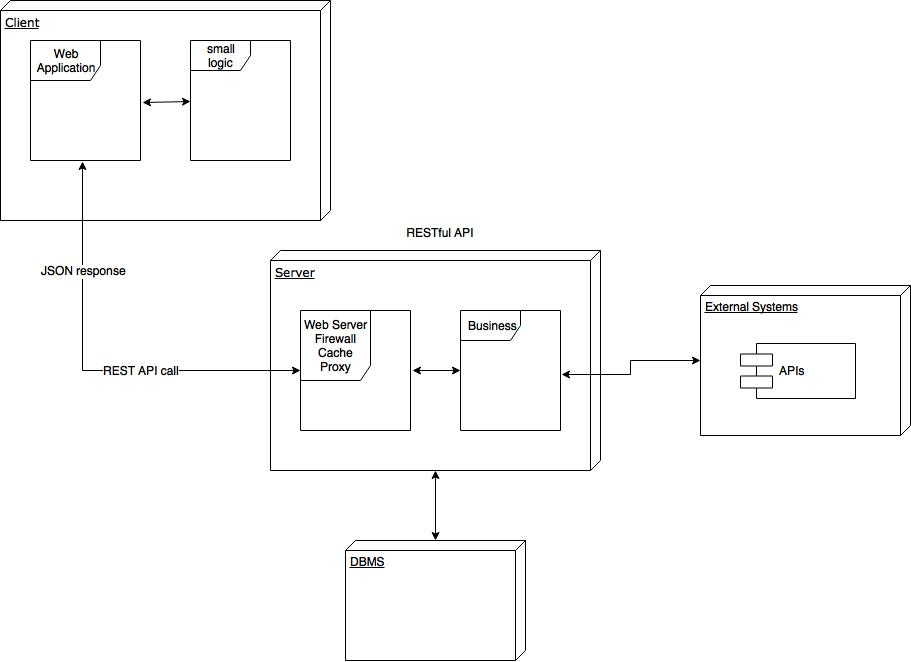
\includegraphics[width=1.2\textwidth]{MainMatter/images/ad/highlevel}}
\captionof{figure}{High level component view of the system}
\end{center}
The client layer will send requests to the server through REST API call. More precisely these requests will be send to the first component of the application layer, the web server. Here the request has to pass through the firewall, then the proxy will direction it to the distributed collection of servers that represents the business layer. The proxy is also in charge to do the opposite communication, when the pieces of information will flow from the business servers, they will have to be directed to the opportune client and the reverse proxy will send to the right client JSON responses.


\begin{landscape}
\begin{center}
\thispagestyle{empty}
\makebox[\textwidth][c]{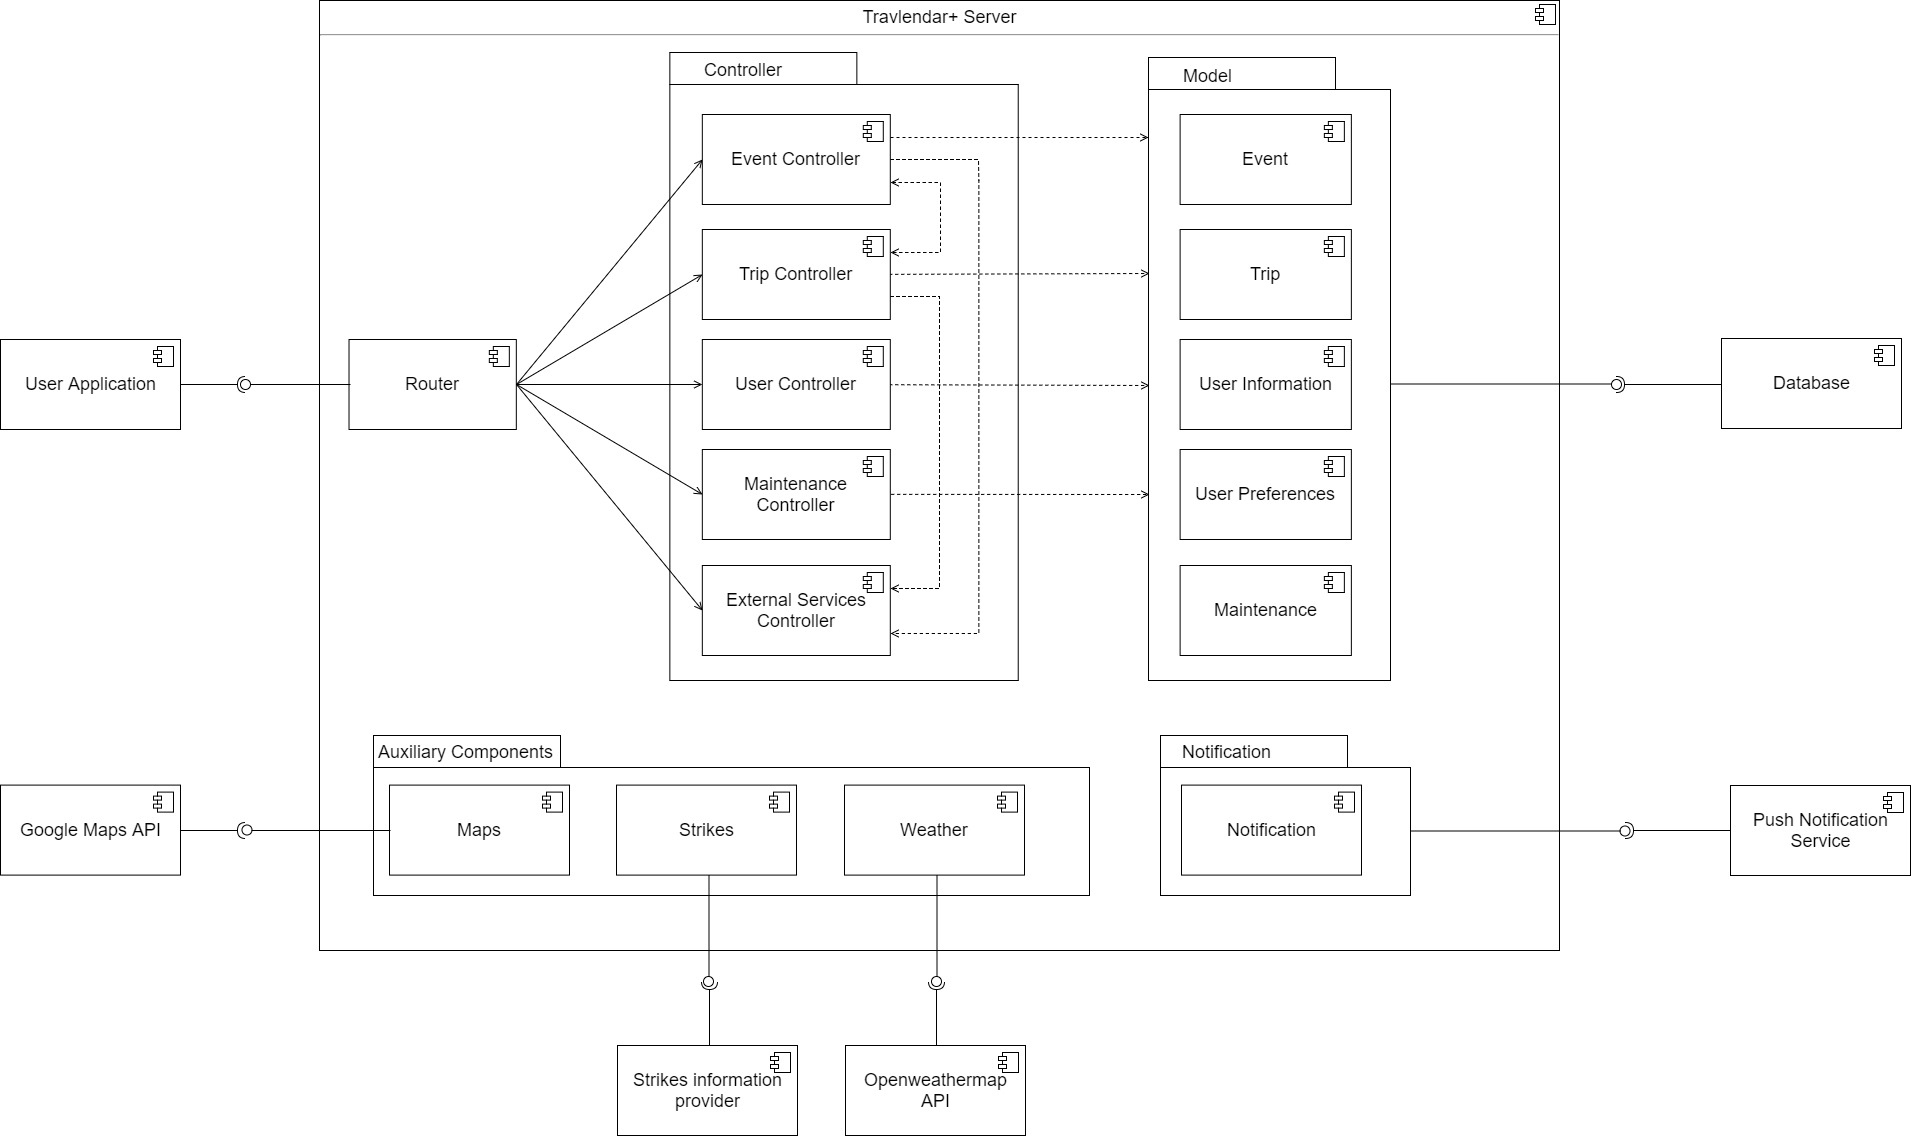
\includegraphics[width=1.55\textwidth]{MainMatter/images/ad/component}}
\captionof{figure}{Component view of the system}
\end{center}
\end{landscape}

The main components are divided in:
\begin{itemize}

\item	Controller set of components
\begin{enumerate}
\item	Event Controller: in charge of the management of events, it will provide functions for adding, modify and delete events and will contain all the logic to do this properly;
\item	Trip Controller: in charge of the management of the trips. It will contain all the necessary logic to avoid overlapping of them and to advise the best option for the user. It also helps the purchase of the tickets;
\item	User Controller: in charge of the management of the user’s info and preferences;
\item	Maintenance Controller: in charge of the management of the maintenance of the system;
\item	External Services Controller: in charge of the management of the external services connected to the system.
\end{enumerate}
\item	Model set of Components are divided in:
\begin{enumerate}

\item	Event: will contain all the information concerning the events;
\item	Trip: will contain all the information concerning the trips;
\item	User Information: will contain all the information concerning the user’s general info;
\item	User Preferences: will contain all the information concerning the user’s preferences;
\item	Maintenance: will contain all the information concerning the maintenance of the system
This layer is strictly connected to the database with which it can exchange data;
\end{enumerate}

\item	Auxiliary Components and Notifications components are:
\begin{enumerate}
\item	Maps: will be connected to the Google Maps API;
\item	Strikes: will be connected to a multitude of APIs from which it will collect all the necessary info;
\item	Weather: will be connected to Open Weather Map API to collect info about weather conditions.
\end{enumerate}
\end{itemize}
It is also present a Router to route request to the appropriate controller.

%
% ------------------------------------------------------------------------ %
%
\section{Deployment View}

\begin{center}
\thispagestyle{empty}
\makebox[\textwidth][c]{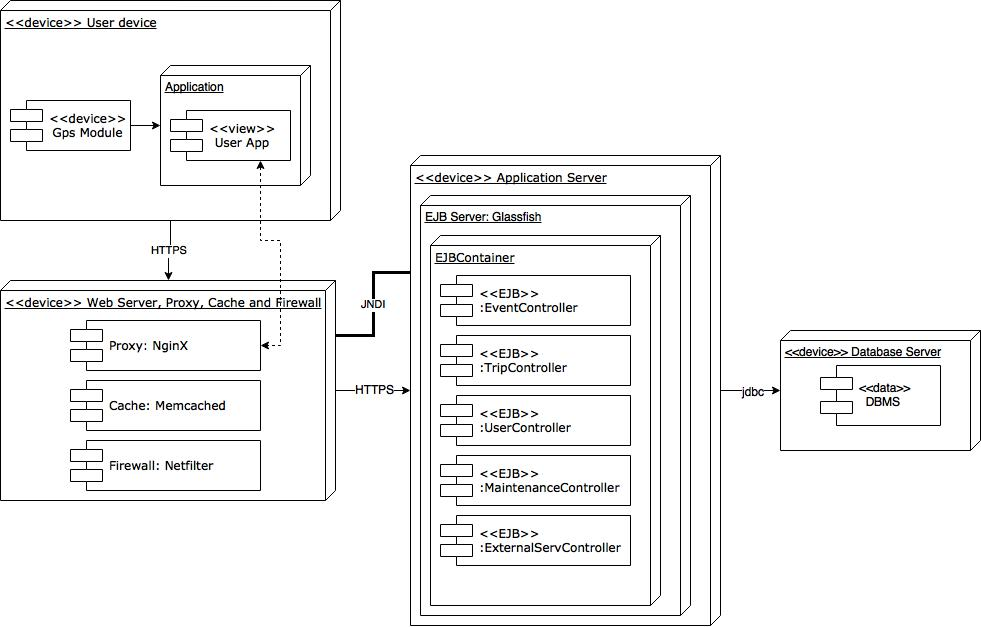
\includegraphics[width=1.2\textwidth]{MainMatter/images/ad/deployment}}
\captionof{figure}{Deployment diagram of the system}
\end{center}

Since our system is subject to several loads concerning data storage and other services we taught that the best deployment solution may be cloud computing, considering also the recent diffusion and opportunity to have access to powerful services with limited costs. 
To be as general as possible and avoid further implementation constraints we prefer to rely on the
IaaS (Infrastructure as a Service) level. It’s specifically a virtualized hardware, in other words an elaboration infrastructure. It includes offers like virtual storage space on servers, network connections, bandwidth and load balancing. Physically, the collection of hardware resources is extracted from several distributed servers and networks usually in different data centres, which maintenance is responsibility of the cloud provider. 
The client, on the other hand, has access to virtualized components to build his IT platforms.
The main advantages are of this approach are:
\begin{itemize}

\item	Scalability: thanks to IaaS upwards and downwards scalability is performed, delays are reduced and waste of resources is prevented;
\item	Costs: base hardware is configured and managed by the cloud provider, therefore no acquisition, installation and maintenance cost are necessary; the cost of the cloud service is almost proportionally to the amount of resource consumed, there are various contracts that allows to design a kind of customized service;
\item	Security: in IaaS configuration, physical security is ensured since it is typically a critical aspect for the provider. In-house security, on the other hand, is not usually an individual’s or an organization’s main business and, therefore, may not be as good as that offered by the IaaS cloud provider;
\item	Availability, Redundancy and Fault Tolerance: deploying different components on different machines allows the system not to totally go down if one of his components crashes. There’s also no need to manage backups because lots of IaaS cloud providers offer automatic backup procedures.
\end{itemize}

On the other hand, some constraints must be respected:
\begin{itemize}
\item	for the scaling mechanism, we have to design stateless components;
\item	we have also do upgrade the developed software;
\item	we have to take care of the maintenance of tools, database systems and the underlying infrastructure.
\end{itemize}
%
% ------------------------------------------------------------------------ %
%
\section{Runtime View}
In this section some sequence diagrams will be presented to describe the interactions that happen between the main components of the system when the most common functionalities are used. This is a high-level description of the actual interactions of the system-to-be, so functions and their names may be added, modified or deleted during the development process.
\\
\\
The functionalities considered for the runtime view are: login, adding of an event on the calendar, trip planning and trip customization.

\pagebreak
\begin{landscape}
\begin{center}
\thispagestyle{empty}
\makebox[\textwidth][c]{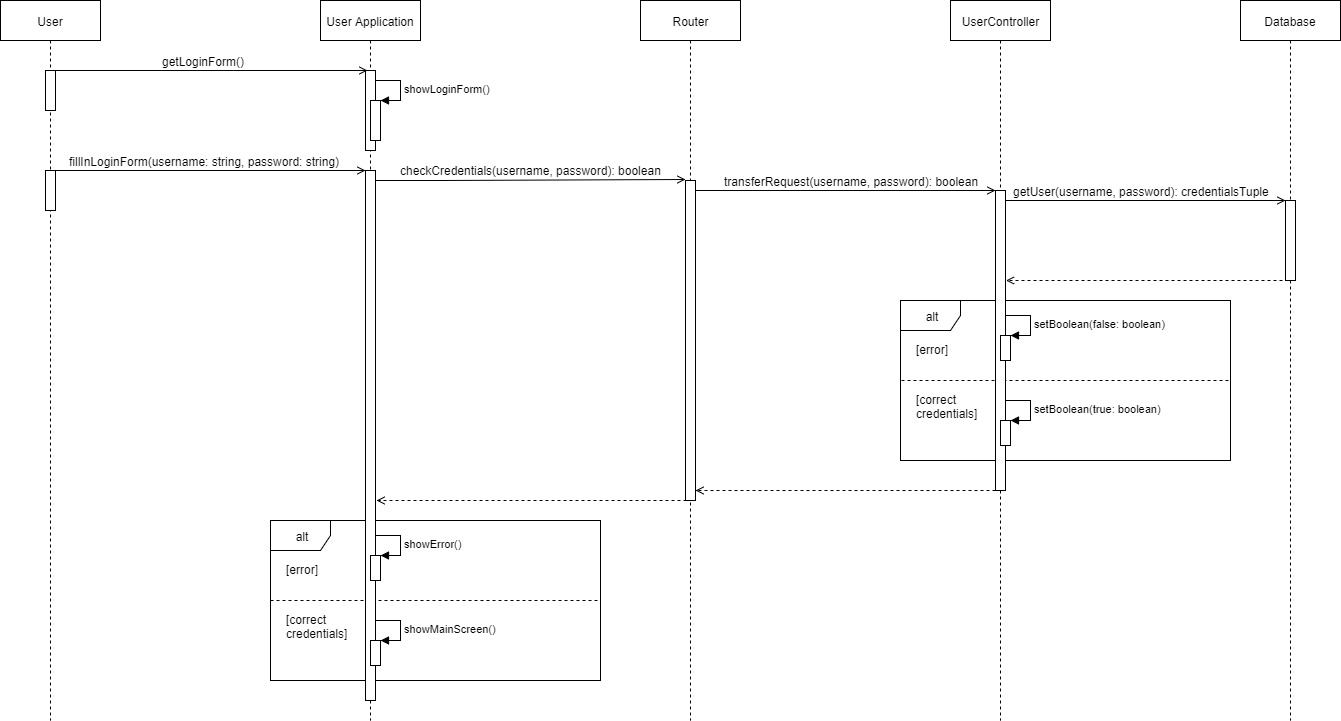
\includegraphics[width=1.76\textwidth]{MainMatter/images/runtime/login}}
\captionof{figure}{User Login runtime view}
\end{center}
\end{landscape}

\pagebreak
\begin{landscape}
\begin{center}
\thispagestyle{empty}
\makebox[\textwidth][c]{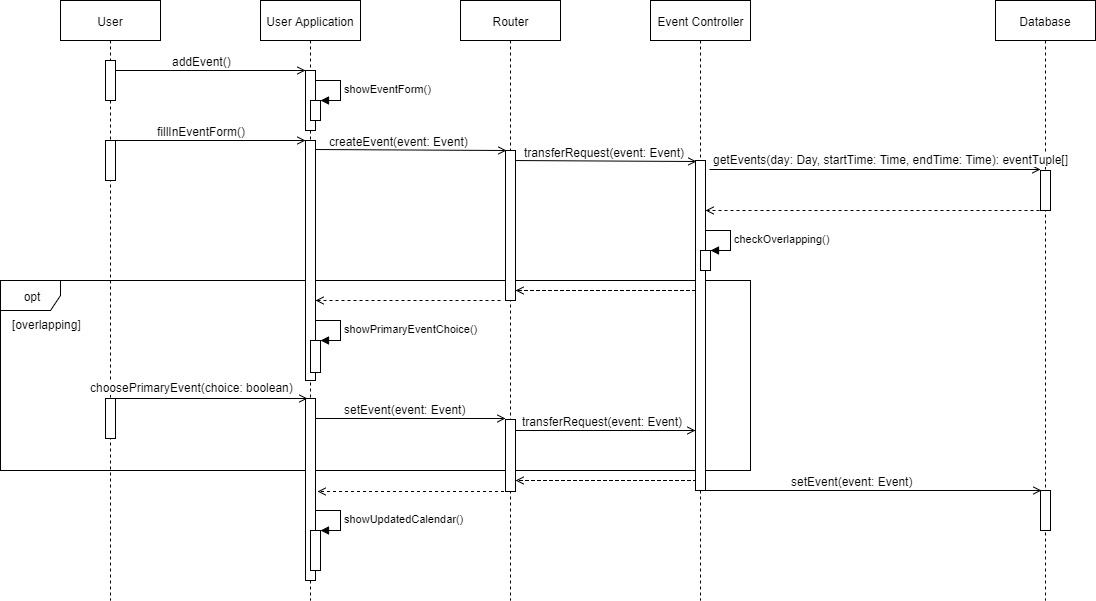
\includegraphics[width=1.72\textwidth]{MainMatter/images/runtime/add}}
\captionof{figure}{Adding of an event in the calendar runtime view}
\end{center}
\end{landscape}

\pagebreak
\begin{landscape}
\begin{center}
\thispagestyle{empty}
\makebox[\textwidth][c]{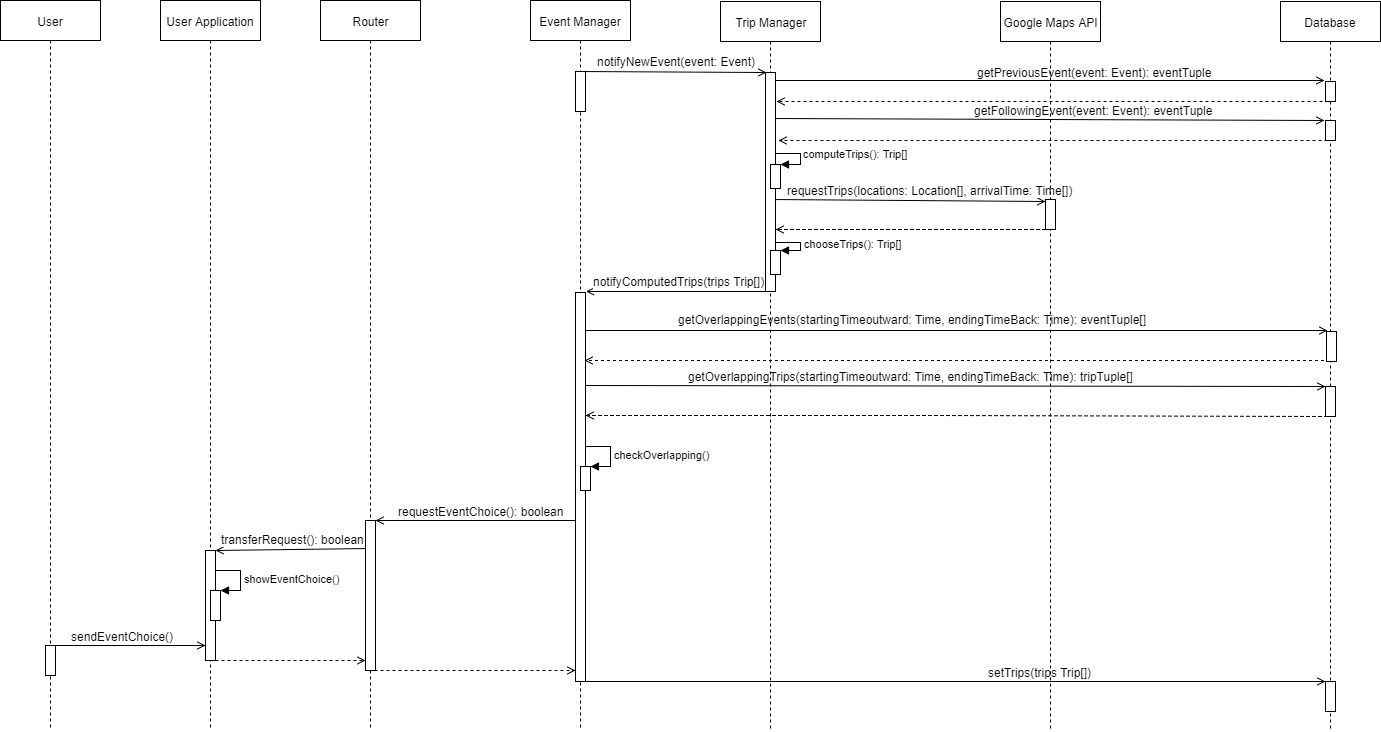
\includegraphics[width=1.78\textwidth]{MainMatter/images/runtime/tripcomm}}
\captionof{figure}{Trip planning runtime view}
\end{center}
\end{landscape}

\pagebreak
\begin{landscape}
\begin{center}
\thispagestyle{empty}
\makebox[\textwidth][c]{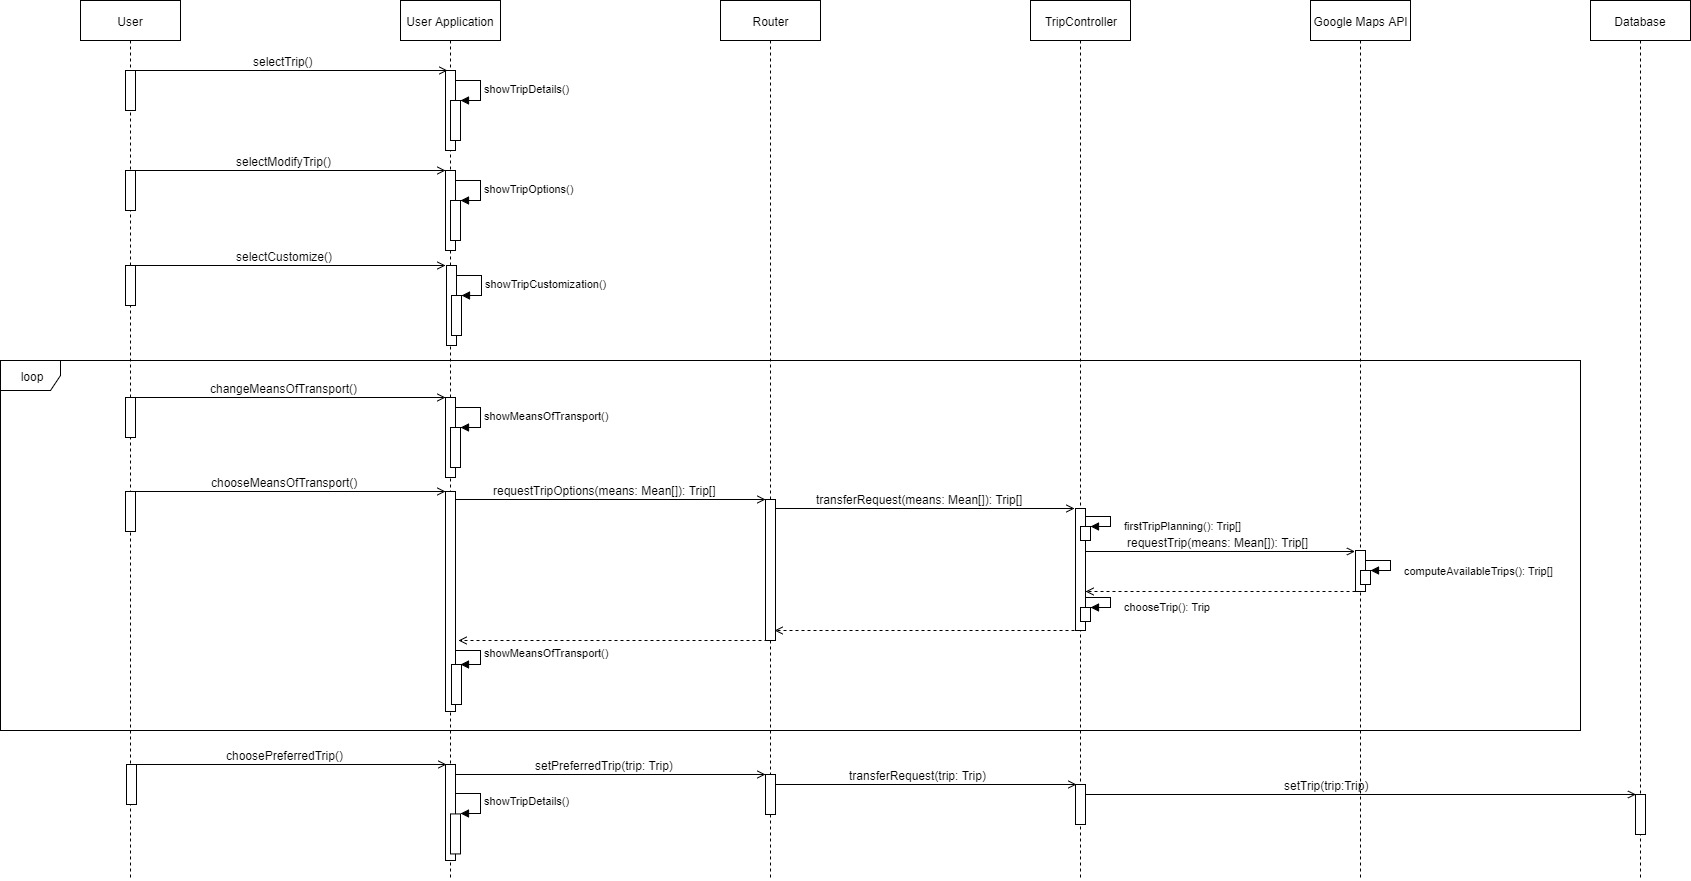
\includegraphics[width=1.81\textwidth]{MainMatter/images/runtime/tripcustom}}
\captionof{figure}{Trip customization runtime view}
\end{center}
\end{landscape}
%
% ------------------------------------------------------------------------ %
%
\section{Component Interfaces}
\begin{itemize}
\item	User Application Interface: responsible for communication between the user application and the application server. The communication will be provided with the HTTPS protocol mostly for security reasons;
\item	Open Weather Map: it gives information about the weather and then the system task will be to compute trips looking also to these pieces of information. For example, if it will be raining it will not suggest a bike trip;
\item	Strikes Information Provider: it gives to our system information about all the possible strikes concerning public means and then it will be the system that will use this information to compute the best travel option for the user;
\item	Google Maps API: it’s used for:
\begin{enumerate}
\item	calculate all the trip times associated to each event, obviously for all types of means (car, bike, public means etc.);
\item	provides information about the traffic to optimize the computation of trip times;
\item	provides the static map that the user will see.
\end{enumerate}
\item	DBMS API: through this the system can retrieve and write data from and to the database. It’s strictly connected to the model through JDBC connector.
\end{itemize}
%
% ------------------------------------------------------------------------ %
%
\section{Selected Architectural Styles and Patterns}

\subsection{Architectural style: Client-Server}
It’s the best known and most used architectural style for distributed applications.
It’s present a well-defined distinction between client and server, they play different roles and also, they are both accessible with a precise interface.
Travlendar+ is a mobile application and will have multiple mobile users, but still the computation portion needs to be located in some point where the global view of the system can be seen.
The system must guarantee scalability so, resources in the form of network segments, computers and servers must be added to the network without major interruptions of it.
Said that, we agreed that the best solution for our needs could be the Client-Server style.
\begin{itemize}
\item	Server is invoked to provide one or a set of services, in our case, for instance, the computation of the best mobility option for the user according to all of his characteristics; 
\item	Clients uses the provided services and initiate the communication through messages or remote invocations. They interact directly with end-users using any user interface such as graphical user interface. These are the user logged in to the application.
\end{itemize}

In the end, we will talk about web clients, which means that in our scenario, they will ask the server to provide services for them and they will not store data locally. Furthermore, the architecture is OS independent, it relies on a central server that will avoid consistency issues between different devices of the same client.

\subsection{Three-tier architecture}
The Client-Server model does not impose any constraint neither about how logical layers (presentation, application/business logic, data) have to be distributed among the deployment units nor about the physical tiers have to be designed.
We taught that the best decision for us could have been the three-tier architecture where each tier is elastically scaled independently. 
That’s composed of:
\begin{itemize}
\item	First tier: Presentation layer located into the mobile application. Handles the interaction with the user. It’s also in charge of some simple validations of the data and the interaction with external systems. Here will be handled all the visualization portion of the system based on the data received from the application layer;
\item	Second tier: web/business layer. Process and executes both new requests of the clients and possible variations on older and not yet completed requests. It will collect information from the users and store them into the databases, but also it will provide to them answers for their requests. 
More precisely, this layer’s tasks are to filter, cache and forwarding the requests between clients and the application server and vice versa. 
It’s also responsible (web layer) of the visualization to the user;
\item	Third tier: Data layer. Dedicated to the storage of information in persistent memory. Data is stored at different locations (replicas) to improve response time and to avoid data loss in case of failures while consistency of replicas is ensured at all times.
\end{itemize}
This architecture permits us to achieve one of the design principles, that says to decouple where possible, in fact we have a solid distinction between logic and data, and also between logic and presentation.

\subsection{Basic architectural patterns}

\subsubsection{Stateless components}
The state is handled external of application components to ease their scaling-out and to make the application more tolerant to component failures. 
In this system cloud resources can display low availability and also component instances can be added and removed regularly when the demand changes.
So, components will be implemented in a way that the do not have any internal state. Instead it will be provided to the component with each request form external persistent storage.

\subsubsection{Stateless components}
An interactive synchronous access to the applications is provided to users, instead the interactions in the application are asynchronous if possible, to ensure loose coupling (Principle 3 of the design principles).
In other words, the user interface component is like a bridge between the synchronous access of the user and the asynchronous communication with other components. Like for stateless components also these ones are obtained from external storage.
The number of components are scaled based on the number of user requests through the elastic load balancer pattern.

\subsubsection{Elastic load balancer}
The number of required components instances is determined by the quantity of synchronous request coming from the users.

\subsubsection{Processing component}
Processing functionalities are divided into separate blocks and assigned to independent processing components each one implemented in a stateless way as explained above.

\subsubsection{Elastic queue}
Queues are used to distribute asynchronous requests to multiple application component instances. From the number of messages queued will be decided the number of component instances handling that requests.

\begin{center}
\makebox[\textwidth][c]{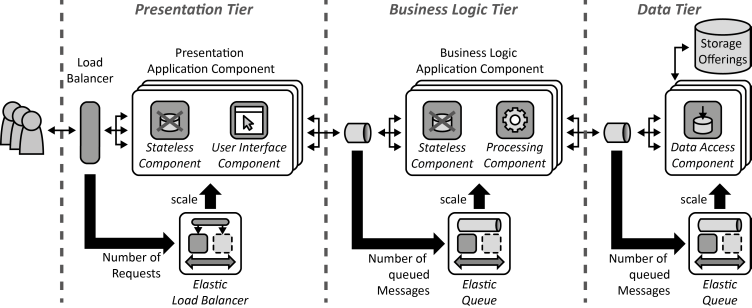
\includegraphics[width=1.2\textwidth]{MainMatter/images/ad/three}}
\captionof{figure}{Three tier cloud application}
\end{center}

\section{Architectural pattern}
\subsubsection{Model View Controller}
The model-view-controller (MVC) design pattern specifies that an application consist of a data model, presentation information, and control information. The pattern requires that each of these be separated into different objects.
\begin{itemize}

\item	The model contains only the pure application data, it contains no logic describing how to present the data to a user, but only data and operations associated to that;
\item	The view presents the model's data to the user. The view knows how to access the model's data, but it does not know what this data means or what the user can do to manipulate it;
\item	The controller exists between the view and the model. It listens to events triggered by the view (so by the user) and executes the appropriate response to these events, usually calling a method on the model and passing the results both to the view and the model.
\end{itemize}
A key aspect is to separate data and its presentation. This not only makes the structure of an application simpler, it also enables code reuse and ensures loose coupling.
It also guarantees the divide and conquer principle allowing parallel development by separated teams in charge of different parts of the application.
\\
An example of how can be represented the MVC pattern is shown in the figure below.

\begin{center}
\makebox[\textwidth][c]{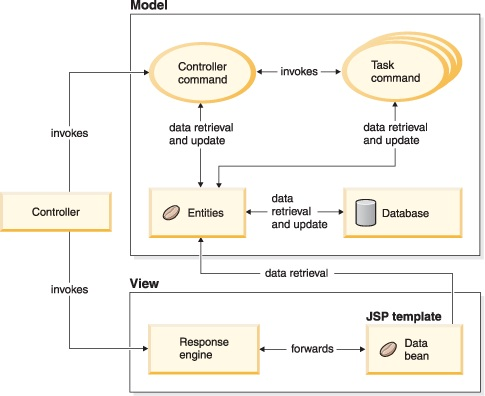
\includegraphics[width=1\textwidth]{MainMatter/images/ad/mvc.jpg}}
\captionof{figure}{Model view controller}
\end{center}

\subsubsection{Commercial architectural system}
To support the development and the execution on enterprise application with a lot of users and lots of requirements we suggest the usage of Java Enterprise Edition (JEE).
That’s a multitier architectural model composed by the client-tier running on the client machine (as we said before in this paragraph, the clients involved in Travlendar+ will be web clients), the business-tier running on the Java EE Server and the enterprise information system (EIS) consisting of databases or other external applications.
This approach will help us also to satisfy non-functional requirements like reliability, performance, security, scalability, availability, extensibility and interoperability. 

The client tier will welcome web clients composed of dynamic web pages, which are generated by web components running in the web tier and a web browser, which renders the pages received
from the business layer.
The application tier will be divided into:
\begin{itemize}

\item	The web layer: in charge of the presentation of the data to the user, it will collect the responses of a client request coming from different servers in the distributed business tier and will send them to the correct user written more likely in JSP or Java Server Faces.
It will also be in charge of firewall, cache, proxy and reverse proxy functions;
\item	The business layer: managing the computing and the execution of the business logic using components called Enterprise Java Beans (EJB) and also interacting with the database through Java Persistence API (JPA).
\end{itemize}
In the end, the Enterprise Information System (EIS) is devoted to the data management and will operate like a DBMS.

\begin{center}
\makebox[\textwidth][c]{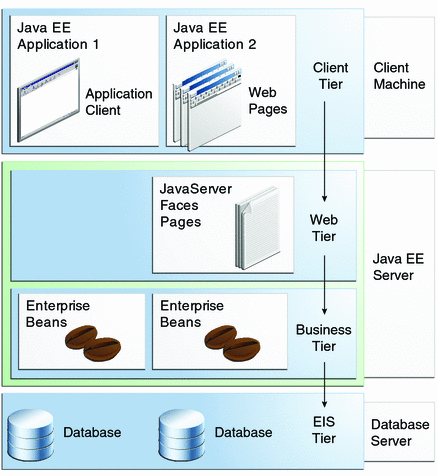
\includegraphics[width=.8\textwidth]{MainMatter/images/ad/commercial}}
\captionof{figure}{ommercial architectural system}
\end{center}
%
% ------------------------------------------------------------------------ %
%
\section{Other Design Decisions}

\subsubsection{Push Notifications}
To send notifications to the Travlendar+ users we choose the Push Notification Technology, obviously supported by iOS and Android.
The APIs we are going to use are:
\begin{itemize}
\item	Apple Push Notification Service for iOS;
\item	Google Cloud Messaging for Android.
\end{itemize}
%
%
% -----------------------------END------------------------------------- %